\documentclass[a4paper,11pt]{article}

\usepackage[margin=3cm]{geometry}

\usepackage{graphicx}
\usepackage{subcaption}
\usepackage[colorlinks,allcolors=violet]{hyperref}
\usepackage{url}
\usepackage{lmodern}

% https://tex.stackexchange.com/questions/94032/fancy-tables-in-latex
\usepackage[table]{xcolor}
\usepackage{booktabs}

\usepackage[utf8]{inputenc}

% https://tex.stackexchange.com/questions/664/why-should-i-use-usepackaget1fontenc
\usepackage[T1]{fontenc}
\usepackage{microtype} % good font tricks

\newcommand{\note}[1]{{\colorbox{yellow!40!white}{#1}}}
\newcommand{\exampletext}[1]{{\color{blue!60!black}#1}}

\begin{document}

\noindent
\colorbox[HTML]{52BDEC}{\bfseries\parbox{\textwidth}{\centering\large
  --- Code review P\&O CW 2019--2020 Task 3 ---
}}
\\[-1mm]
\colorbox[HTML]{00407A}{\bfseries\color{white}\parbox{\textwidth}{
  Department of Computer Science -- KU Leuven
  \hfill
  \today
}}
\\

\smallskip

\noindent
%\mbox{}\hfill
\begin{tabular}{*4l}
\toprule
\multicolumn{3}{l}{\large\textbf{Team 12}} \\
\midrule
Martijn Debeuf & 2.5h & 750 LOC \\ % fill in the time spend on this task per team member who worked on it and the amount of lines of code (LOC) reviewed
Frédéric Blondeel & 2h & 650 LOC \\
\bottomrule
\hline
\end{tabular}\\
\\
Demo: \url{https://penocw.cs.kotnet.kuleuven.be:80##/demo-task-44?0xjwkkslam9} \\
Files reviewed: barcodeScanner/main.js; screenDetection/main.js; screenDetection/image.js

\noindent
{\color[HTML]{52BDEC} \rule{\linewidth}{1mm} }

\smallskip

\begin{itemize}

\item Bij de file Image.js is nog geen commentaar toegevoegd, dit maakt het lezen en begrijpen van de code lastig.
\item Bij de changeColorspace() methode kan misschien een array bijgehouden worden met de toegelaten colorspaces als soort van veiligheid of indien er effectief maar twee gebruikt worden is het misschien beter om deze als een boolean bij te houden. 
\item Het verschil tussen de methode getImgData() en show() is niet erg duidelijk, kan ook verholpen worden door commentaar te voorzien.
\item De screenDetection/main.js code moet nog mooier geordend worden maar dit wordt momenteel nog als test gebruikt. De andere bestanden zijn simpele code waar niet veel over op te merken is.
\item In cornerDetection() zijn de if-voorwaarden uit de lucht gevallen, er is geen reden dat deze 7 en niet 8 is bijvoorbeeld (zie figuur).

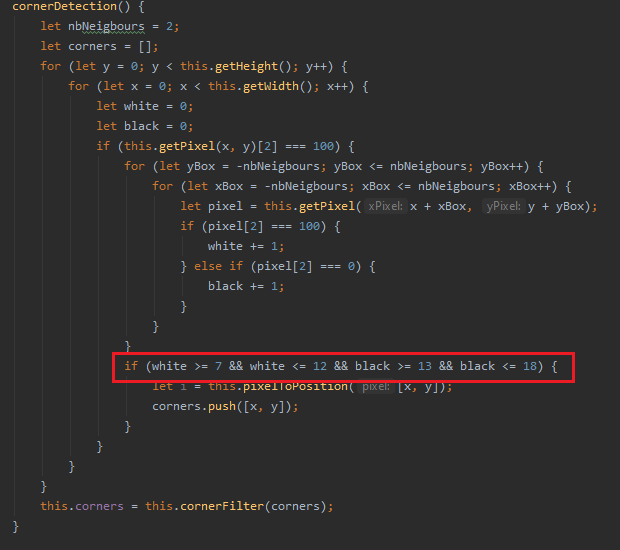
\includegraphics[scale=0.75]{code1}
\item De floodfill(), calcIslandsFloodfill() en calcIslands() zijn moeilijk te begrijpen. Documentatie is hier essentieel want deze zijn complexe functies. Ook meer uitleg in verband met workMatrix is nodig want deze komt uit het niets tevoorschijn.


\end{itemize}





\end{document}